\documentclass[twoside,11pt,a4paper]{article}

\usepackage[utf8]{inputenc}
\usepackage{latexsym,amsmath,amssymb}
\usepackage{ngerman}
\usepackage{theorem}
\usepackage{dcolumn}
\usepackage{url}
\usepackage{tikz}
\usepackage[hidelinks]{hyperref}
\usetikzlibrary{trees,calc}

\newcommand{\Frac}[2]{\frac{\displaystyle #1}{\displaystyle #2}}
\newlength{\textwd}
\newlength{\oddsidemargintmp}
\newlength{\evensidemargintmp}
\newcommand{\hspaceof}[2]{\settowidth{\textwd}{#1}\mbox{\hspace{#2\textwd}}}
\newlength{\textht}
\newcommand{\vspaceof}[3]{\settoheight{\textht}{#1}\mbox{\raisebox{#2\textht}{#3}}}
\newcommand{\PreserveBackslash}[1]{\let\temp=\\#1\let\\=\temp}

\newenvironment{deflist}[1][\quad]%
{  \begin{list}{}{%
      \renewcommand{\makelabel}[1]{\textbf{##1}\hfil}%
      \settowidth{\labelwidth}{\textbf{#1}}%
      \setlength{\leftmargin}{\labelwidth}
      \addtolength{\leftmargin}{\labelsep}}}
{  \end{list}}

\newenvironment{Quote}% Definition of Quote
{  \begin{list}{}{%
      \setlength{\rightmargin}{0pt}}
      \item[]\ignorespaces}
{\unskip\end{list}}

\newtheorem{Cor}{Corollary}
\theoremstyle{break}
\theorembodyfont{\itshape}
\newtheorem{Def}[Cor]{Definition}
\theoremheaderfont{\scshape}

\newcolumntype{.}{D{.}{.}{-1}}

\pagestyle{headings}

\textwidth 15cm
\textheight 23cm
\oddsidemargin 1cm
\evensidemargin 0cm

\tikzset{
grow=down,
level 1/.style={sibling distance=2.5cm, level distance=1.0cm},
level 2/.style={sibling distance=1cm, level distance=1.0cm},
level 3/.style={sibling distance=1cm, level distance=1.5cm},
edge from parent path={
(\tikzparentnode) |-
($(\tikzparentnode)!0.5!(\tikzchildnode)$) -|
(\tikzchildnode)}
}

% Define styles for bags and leafs
\tikzstyle{bag} = [text width=8em, text centered]
\tikzstyle{cicleend} = [circle, minimum width=3pt, fill, inner sep=0pt]

\begin{document}

\pagestyle{empty}
\begin{center}
    Rheinisch-Westfälische Technische Hochschule Aachen \\
    Lehrstuhl für Informatik VI \\
    Prof. Dr.-Ing. Hermann Ney\\[6ex]
    Proseminar Datenkompression im WS 2014/2015\\[12ex]

    \LARGE
    \textbf{Adaptive Huffman-Kodierung und Anwendungen} \\[6ex]
    \textit{Thomas Gatzweiler} \\[6ex]
    \Large
    Matrikelnummer 318947 \\[6ex]
    12. November 2014

    \vfill
    \Large Betreuer: Patrick Dötsch
\end{center}

\newpage
\
\newpage

\pagestyle{headings}
\tableofcontents
\listoftables
\listoffigures
\newpage
\pagestyle{empty}
\
\newpage
\pagestyle{headings}


\setlength{\parindent}{0pt}
\setlength{\parskip}{2ex plus 0.5ex minus 0.2ex}

% Literaturverzeichnis wie in der .bib Datei ordnen
\nocite{*}

\section{Einleitung}

Bei einer Datenübertragung mit eingeschränkter Bandbreite ist eine Komprimierung
der Daten von großem Vorteil.

Ein Problem der Huffman-Kodierung ist, dass die Wahrscheinlichkeiten der
Quellsymbole vor der Kodierung bekannt sein müssen. Wenn die zu komprimierenden
Daten lokal verfügbar sind, ist es möglich, zuerst die Häufigkeiten der
vorkommenden Quellsymbole zu analysieren und dann die Daten zu kodieren. Handelt
es sich aber um einen laufenden Datenstrom, ist es nicht möglich die Häufig im
vorraus zu ermitteln. Eine Lösung für dieses Problem bietet die adaptive
Huffman-Kodierung, die sich laufend an die Häufigkeiten der Quellsymbole
anpasst.

\section{Huffman-Kodierung}

Dieser Abschnitt gibt eine Einführung in die Hufmann-Kodierung, auf welche die
adaptive Huffman-Kodierung aufbaut. Der Abschnitt basiert auf \cite[S.
214-228]{Salomon:2010}.

Die Huffman-Kodierung ist eine stochastische Kodierung, das heißt, sie kodiert
Daten basierend auf der Häufigkeit der vorkommenden Quellsymbole. Häufig
vorkommenden Symbolen wird ein kürzeres Codewort zugewiesen als selteneren
Symbolen.

Es gibt Fälle, in denen durch die Huffman-Kodierung keine Komprimierung erziehlt
werden kann. Zum Beispiel mit den Quellsymbolen 0 und 1 und der Folge
{\tt01010101}. Beide Quellsymbole haben eine Wahrscheinlichkeit von 50\%,
deshalb bekommen sie beide ein Codewort der Länge 1 zugewiesen.

\subsection{Huffman-Baum}

Um Daten mit der Huffman-Kodierung zu komprimieren muss zuerst der sogenannte
\emph{Huffman-Baum} aufgebaut werden. Es handelt sich dabei um einen Binärbaum,
der einigen Bedingungen unterliegt.

Der Huffman-Baum wird von unten nach oben Aufgebaut, also von den Blättern zur
Wurzel. Jedes Blatt steht für ein Quellsymbol. Aus dem Pfad zu einem Blatt lässt
sich das Codewort für dieses Blatt ableiten.

% sibling-property


\begin{figure}
\centering
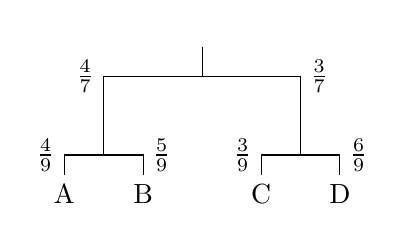
\begin{tikzpicture}
\node {}
    child {
            child {
                node {A}
                edge from parent
                node[left]  {$\frac{4}{9}$}
            }
            child {
                node {B}
                edge from parent
                node[right]  {$\frac{5}{9}$}
            }
            edge from parent
            node[left]  {$\frac{4}{7}$}
    }
    child {
        child {
                node {C}
                edge from parent
                node[left] {$\frac{3}{9}$}
            }
            child {
                node {D}
                edge from parent
                node[right] {$\frac{6}{9}$}
            }
        edge from parent
        node[right] {$\frac{3}{7}$}
    };
\end{tikzpicture}
\caption{M1} \label{fig:M1}
\end{figure}

\subsection{Kodierung}
Nachdem der Huffman-Baum generiert wurde, kann er zur Kodierung von Daten
verwendet werden.

\subsection{Dekodierung}
Auch für die Dekodierung wird der Huffman-Baum verwendet. Dazu muss der
Dekodierer die Häufigkeitsverteilung der Quellsymbole kennen

\subsection{Mittlere Codewort-Länge}

\subsection{Höhe des Baumes}

Da die Höhe des Huffman-Baumes der maximalen Codewort länge entspricht,
ist die Berechnung von Interesse.

\section{Adaptive Huffman-Kodierung}

Die adaptive Huffman-Kodierung aktualisiert laufend den Huffman-Baum.

Da anfangs noch keine Häufigkeiten der auftauchenden Wörter Symbole bekannt
sind, wird mit einem leeren Baum begonnen. Mit jeden neuen Wort wird der Baum
entsprechend der neuen Wahrscheinlichkeitsverteilung aktualisiert. Dieser
Schritt wird auch im Dekodierer durchgeführt, so dass eine Übertragung des
Huffman-Baums nicht nötig ist.

Der Vorteil der adaptiven Huffman-Kodierung ist die Möglichkeit einen Datenstrom
zu komprimieren ohne vorher Informationen über die Häufigkeitsverteilung der
Daten zu besitzen. Das macht es auch möglich Dateien in nur einem Durchgang zu
komprimieren, ohne voher die Häufigkeiten der vorkommenden Wörter zu
analysieren. Ein Nachteil ist, dass diese Methode anfällig für
Übertragungsfehler ist, da die Hufmann-Bäume im Encoder und Decoder in diesem
Fall divergieren können.

\subsection{Kodierung}

\subsection{Dekodierung}

\subsection{Aktualisierung des Huffman-Baums}

% Beispiel

\subsection{Überlauf der Häufigkeitszähler}

Die Häufigkeitszähler für das Auftreten von Quellsymbolen werden bei der
adaptiven Huffman-Kodierung als Integer gespeichert. Abhängig von der Datenmenge
kann es passieren, dass die auftretende Häufigkeit eines Symbols die Grenze des
darstellbaren Zahlenbereiches überschreitet -- es kommt zu einem
Integerüberlauf.

Der darstellbare Zahlenbereich für Integer ist abhängig von der verwendeten
Hardware. Mit modernen 64-Bit Rechnerarchitekturen ist die Wahrscheinlichkeit
für einen Überlauf heute deutlich geringer, die Möglichkeit sollte dennoch nicht
vernachlässigt werden. Viele Microcontroller rechnen standardmäßig mit 8- oder
16-Bit-Integern, die nur 256 bzw. 65536 Werte darstellen können.

Eine Möglichkeit zu Verhinderung der Überläufe wäre die Benutzung einer
Biblitothek zur Speicherung von Integern mit dynamischer Größe, wie zum Beispiel
die \emph{GNU Multiple Precision Arithmetic Library}\cite{GMP}. Ein Nachteil ist
der entstehende Overhead, außerdem ist die Verwendung einer solchen Bibliothek
bei vielen Microcontrollern nicht möglich.

Eine weitere Methode gegen das Überlaufproblem ist das Prüfen auf einen
möglichen Überlauf wenn ein Häufigkeitszähler inkrementiert wird. Würde durch
das Inkrementieren eines Zählers ein Überlauf entstehen, werden alle
Häufigkeitszähler neu skaliert. Dafür werden zunächst die Häufigkeitszähler
aller Blätter des Huffman-Baums durch 2 dividiert, was einer einfachen
Rechtsshift-Operation enstpricht. Dann werden von den Blättern ausgehend bis zu
Wurzel die Zähler aller Zwischenknoten mit der Summe der Kinderknoten
aktualisiert.

Da durch die Integer-Divison Genauigkeit verloren geht, kann es passieren, dass
der resultierende Baum kein Huffman-Baum mehr ist. Die Lösung dafür ist die
vollständige Neuerstellung des Huffman-Baums nach jeder Skalierung. Aber Selbst
bei der Verwendung von 32-Bit Integern sollte dies nicht sehr häufig passieren.

% Beispiel

Die Skalierung der Zähler hat eine Auswirkung auf die Komprimierung, denn die
Symbole, die nach der Skalierung gelesen werden, haben eine größere Auswirkung
auf die Häufigkeitszähler, als die Symbole vorher, deren Wert halbiert wurde.
Dies kann sogar einen Vorteil haben, denn die neu gelesenen Symbole können eine
größere Abhängigkeit von den kurz vohrer aufgetretenen Symbolen haben als von
Symbolen, die weiter in der Vergangenheit aufgetreten sind.

\subsection{Überlauf der Codeworte}

Wie in Abschnitt xy beschrieben, wird die maximale Länge eines Codeworts
von der Höhe des Huffman-Baums bestimmt.

% -> Salomon 5.2.7 Height of a Huffman Tree
% Betrifft nur den Kodierprozess

\subsection{Algorithmus von Vitter}

\section{Anwendungen}

In der Praxis wird die Huffman-Kodierung in der adaptiven Variante zum Beispiel
im Unix-Tool \emph{compact} verwendet. Bei vielen anderen Programmen ist die
Huffman-Kodierung Teil eines mehrstufigen Prozesses der Komprimierung.

% -> Salomon 5.2.9 Is Huffman Coding Dead

Die hier vorgestellten Anwendungsfälle basieren auf den Beispielen aus
\cite{Sayood:2006}.

% -> Sayood 3.8 Applications of Huffman Coding
\subsection{Textkomprimierung}

\subsection{Verlustfreie Bildkomprimierung}

\subsection{Audiokomprimierung}


Test \cite{Salomon:2010}  \cite{Williams:1991}

\addcontentsline{toc}{section}{Literaturverzeichnis}
\bibliographystyle{unsrt}
\bibliography{adaptive_huffman}

\end{document}
